\documentclass[11pt]{article}
\usepackage{epsfig}
\usepackage{alltt}
\usepackage{amsmath}
\usepackage{multicol}
\usepackage{wrapfig}			% For figure text wrapping
\usepackage{graphicx}			% For including graphics
\usepackage{float}
\usepackage{subfigure}			% For subfigures
\usepackage{tabularx}			
\usepackage{fancy headings}		% For header and footers

\marginparwidth 0pt
\oddsidemargin  0pt
\evensidemargin  0pt
\marginparsep 0pt
\parindent 0pt
\parskip 7.2pt

\topmargin   -0.5in

\textwidth   6.5in
\textheight  9 in

\pagestyle{fancy}

% Header:
\fancyhead{}
\lhead{Speaker Building}
\chead{}
\rhead{}

% Footer:
\fancyfoot{}
\lfoot{MET-lab}
\cfoot{\thepage}
\rfoot{Drexel University}

%%% BEGIN DOCUMENT
\begin{document}

{\bf \LARGE Energy Transduction: Building a Speaker}

You will be working in groups of 2-3 students to construct your speaker. 

{\bf Please be careful with the magnets. These neodymium magnets are very powerful and can break or injure you if they snap together from a distance. Keep them at least one foot away from computers, credit cards, and other electronic devices as they can interfere with magnetic storage.}

\section*{Materials}		

\begin{figure}[htb]\center
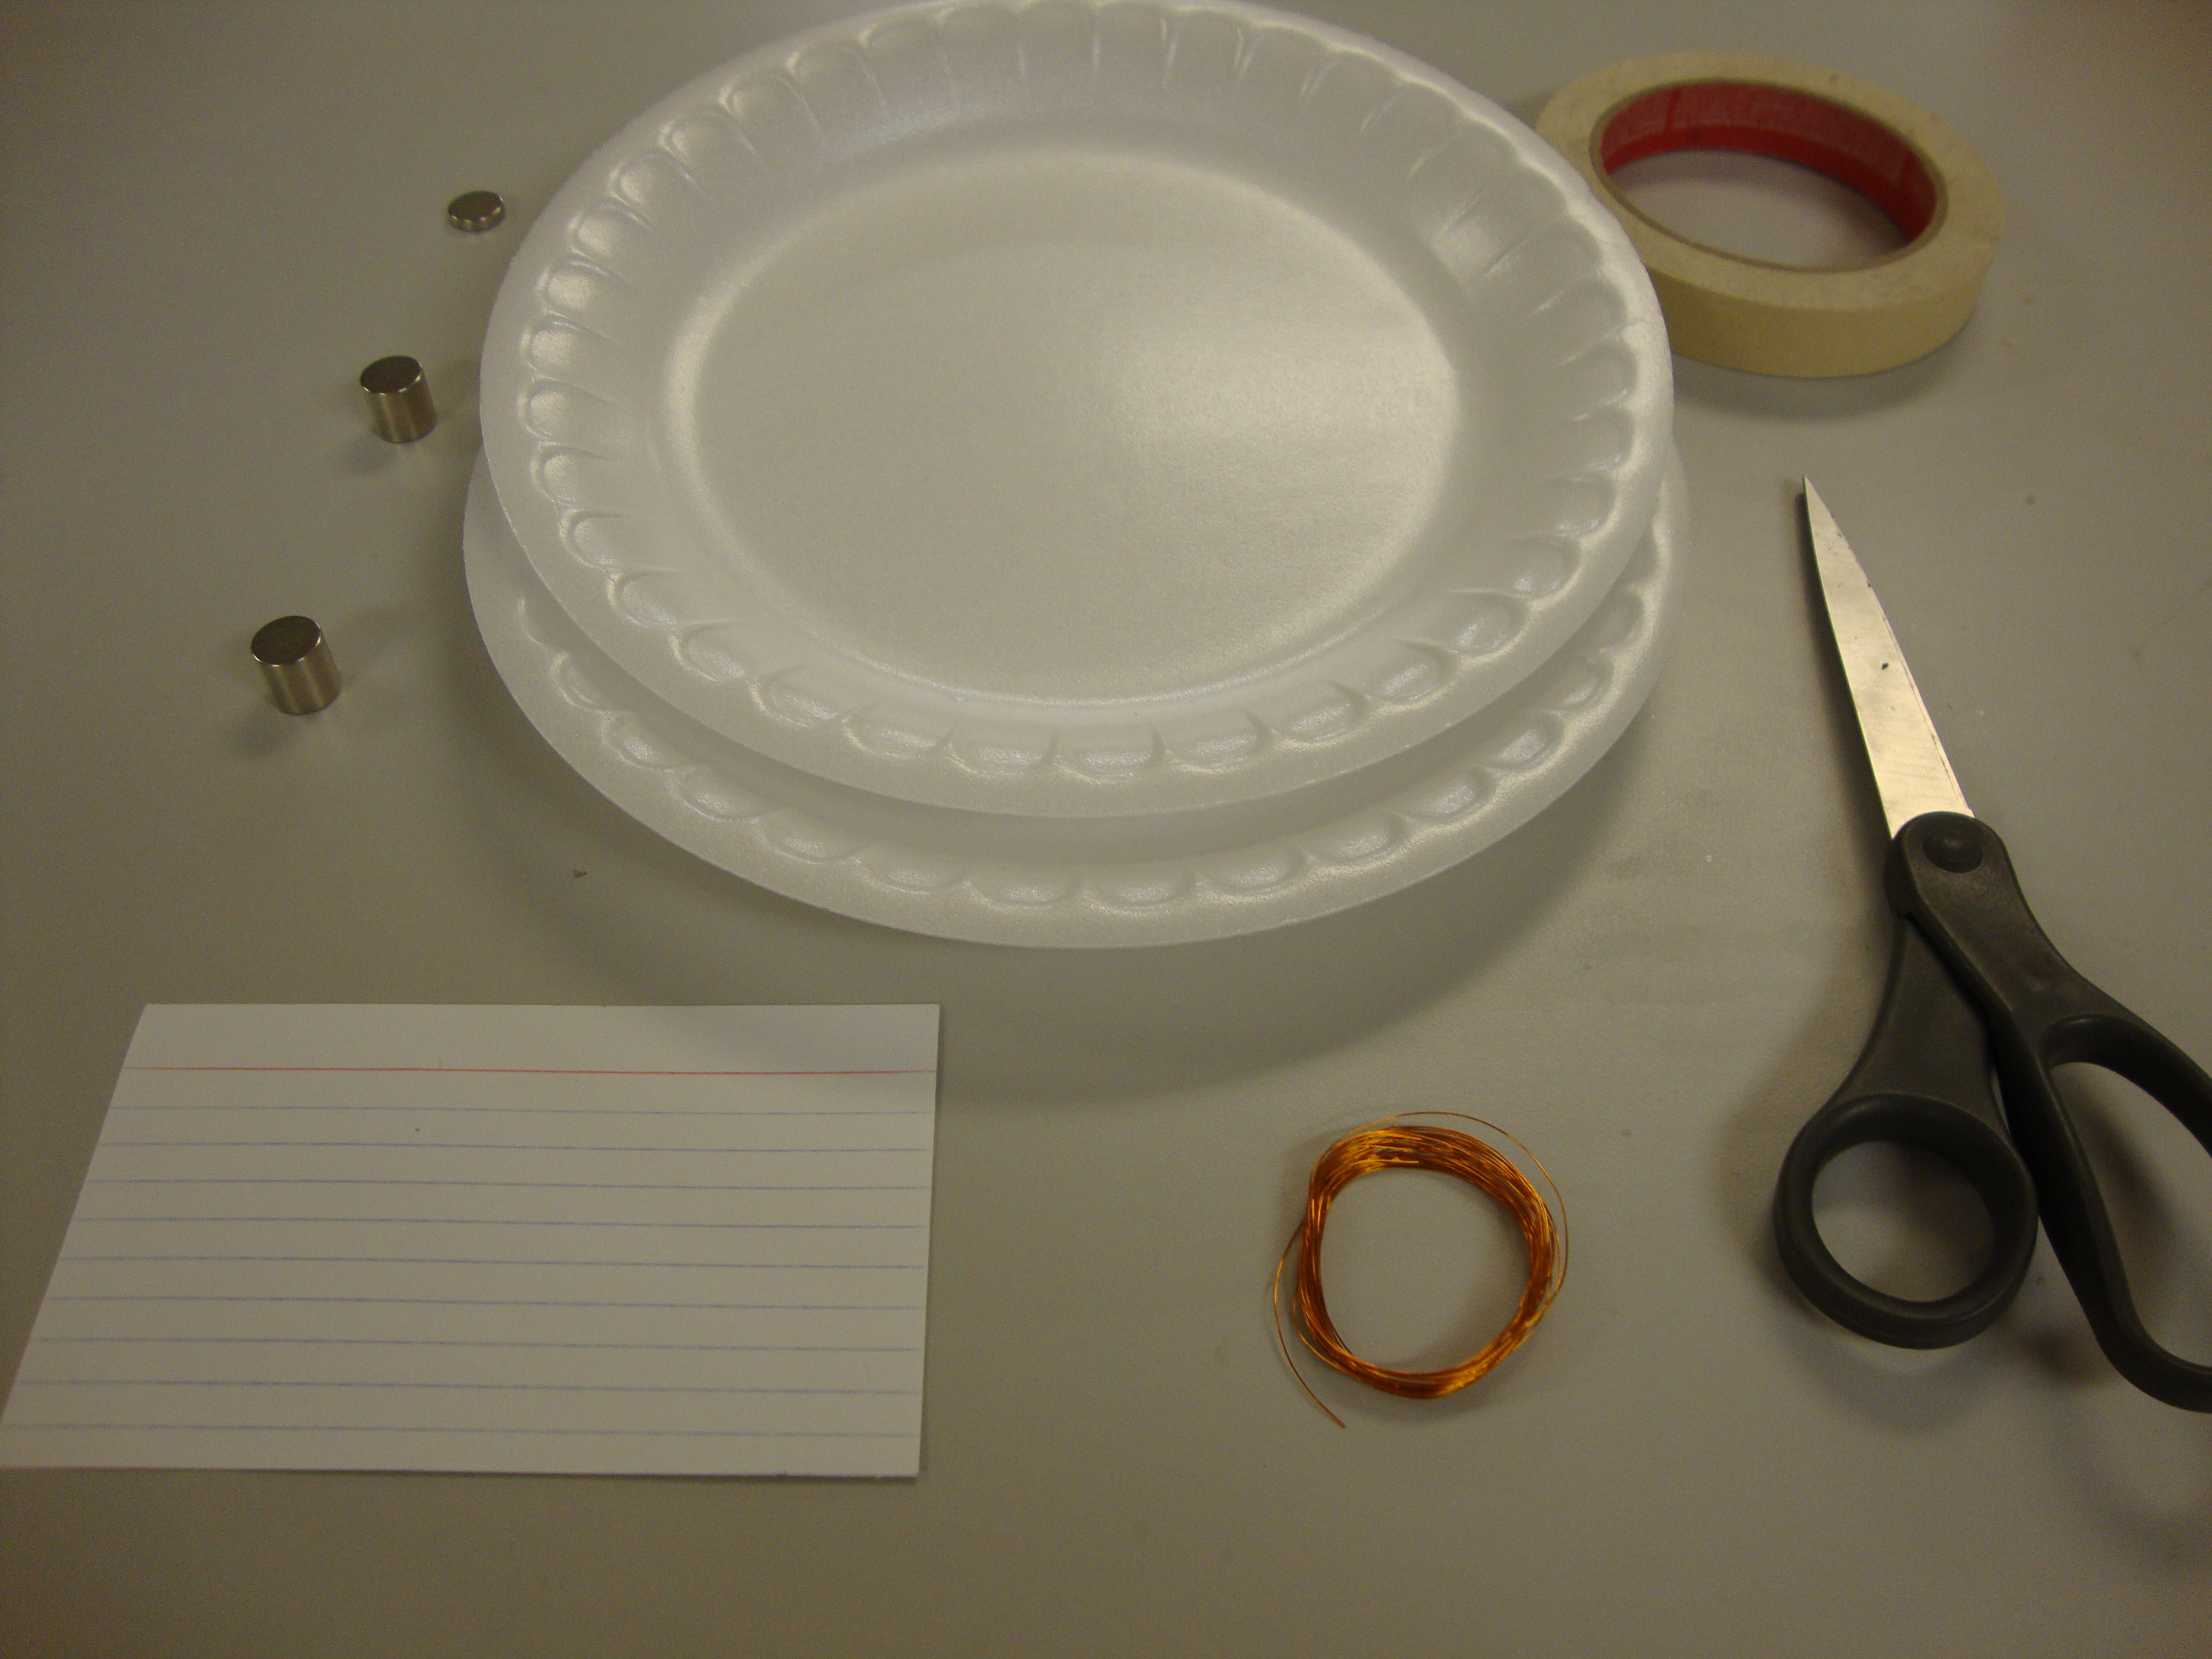
\includegraphics[width=0.8\textwidth]{images/DSC00407.pdf}
\caption{Materials for our loudspeaker}
\label{fig:materials}
\end{figure}

\begin{itemize}
	\item 2 Cylindrical neodymium magnets 1/2" diameter x 1/2" height
	\item 1 Cylindrical neodymium magnet 1/2" diameter x 1/8" height
	\item 2 Paper or styrofoam plates
	\item 1 Index card
	\item $\approx$17 feet of 30 gauge magnet wire
	\item Masking tape
	\item Scissors
\end{itemize}

\newpage

\section*{Winding the "Voice Coil"}			% Coil winding

\vspace{0.5cm}

\begin{figure}[H]
	\begin{minipage}[b]{0.69\linewidth}
		\centering	\includegraphics[width=\textwidth]{images/coil_frame.pdf}
	\end{minipage}
	\hspace{0.1cm}
	\begin{minipage}[b]{0.3\linewidth}
		\begin{enumerate} \setcounter{enumi}{0}
			\item Cut off about a third off the length off the index card and roll it around your finger.
			\item Use the magnets to size the coil frame. There should be about a 1/8" gap between magnet and coil. Tape the coil 					frame in place.
		\end{enumerate}
	\end{minipage}
\end{figure}

\vspace{1.8cm}

\begin{figure}[H]
	\begin{minipage}[b]{0.69\linewidth}
		\centering	\includegraphics[width=\textwidth]{images/wind_coil.pdf}
		\vspace{1.2cm}
	\end{minipage}
	\hspace{0.1cm}
	\begin{minipage}[b]{0.3\linewidth}
		\begin{enumerate} \setcounter{enumi}{2}
			\item {\bf Leaving an extra 4-5" of wire on each end}, wind the coil around the frame, starting in the middle and working 					toward one end.  \\ \\
				{\bf Use $\geq 70$ turns!}
				{\bf Record the number of turns you used below.} \\ \\ 
				$\#$Turns: \hrulefill
		\end{enumerate}
	\end{minipage}
\end{figure}

\vspace{0.5cm}

\begin{figure}[H]
	\begin{minipage}[b]{0.6\linewidth}
		\centering	\includegraphics[width=\textwidth]{images/scrape.pdf}
	\end{minipage}
	\hspace{0.1cm}
	\begin{minipage}[b]{0.45\linewidth}
		\begin{enumerate} \setcounter{enumi}{3}
			\item Secure the ends of the voice coil with masking tape. You could also put small pieces of tape on the end of the coil 					frame to keep the coil from slipping over and unwinding.
			\item {\bf Very important:} Scrape the enamel layer off the ends of the voice coil. This allows you to make a connection to 				the bare copper wire.
		\end{enumerate}
	\end{minipage}
\end{figure}

\newpage

\section*{Assembling the Speaker}			% Assembly

\begin{figure}[H]
	\begin{minipage}[b]{0.69\linewidth}
		\centering	\includegraphics[width=\textwidth]{images/plates.pdf}
	\end{minipage}
	\hspace{0.1cm}
	\begin{minipage}[b]{0.3\linewidth}
		\begin{enumerate} \setcounter{enumi}{5}
			\item Tape the coil in the center of a plate. 
			\item Place the two larger magnets in the center of the other plate. Use the smaller magnet on the plate's underside to hold 				the magnets in place.			
		\end{enumerate}
	\end{minipage}
\end{figure}

\vspace{1.6cm}

\begin{figure}[H]
	\begin{minipage}[b]{0.69\linewidth}
		\centering	\includegraphics[width=\textwidth]{images/spiders.pdf}
	\end{minipage}
	\hspace{0.1cm}
	\begin{minipage}[b]{0.3\linewidth}
		\begin{enumerate} \setcounter{enumi}{7}
			\item Cut the remaining piece of index card in half and fold the halves into a 'W' shape, these will be your supports.
			\item Tape them at opposite ends of the plate. You can add more for increased stability as shown.		
		\end{enumerate}
	\end{minipage}
\end{figure}

\vspace{1.6cm}

\begin{figure}[H]
	\begin{minipage}[b]{0.4\linewidth}
		\centering	\includegraphics[width=\textwidth]{images/finished.pdf}
	\end{minipage}
	\hspace{0.1cm}
	\begin{minipage}[b]{0.59\linewidth}
		\begin{enumerate} \setcounter{enumi}{9}
			\item Finally, attach the top plate to the bottom plate. Carefully adjust the magnets (don't rip the plate) so that they sit directly 				underneath the coil, and the magnet does not touch the coil frame.
			
				You will likely need to make adjustments to the suspension so that bottom of the coil sits in an equilibrium position $				\approx 1cm$ from the bottom plate. 
			\vspace{1.5cm}
		\end{enumerate}
	\end{minipage}
\end{figure}

\begin{enumerate} \setcounter{enumi}{10}
	\item When you are finished constructing your speaker, bring it to an instructor to connect it to an amplifier for testing.
\end{enumerate}

\newpage

\section*{Questions for Inquiry (and Follow-up Discussion)}

How does your speaker sound? Is it quiet or loud? Is it distorted or clear?
\\ \\ \\ \\ \\ \\ \\ \\ \\ \\
Is the speaker reproducing all frequencies (pitches) equally, or does it not work well in certain ranges?
\\ \\ \\ \\ \\ \\ \\ \\ \\ \\
Mount your voice coil on a plate of a different material and note any changes in the sound (volume/clarity).
\\ \\ \\ \\ \\ \\ \\ \\ \\ \\
You can try to make more than one coil if you have time.  Significantly increase the number of turns and see how the sound is affected.

\newpage

\section*{Background: Transduction}			%% Background 
In this activity, we are exploring the basics of {\bf transduction}, which in its most general sense is a conversion of one form of energy to another. More specifically, we'll be dealing with {\bf audio transducers}, devices which convert {\bf sound pressure} to {\bf electrical signals} and vice-versa. Examples of audio transducers include {\bf microphones} and {\bf loudspeakers}. In this activity, we build a loudspeaker from some magnets, wire, and household materials.

\begin{figure}[H]
   \centering
   \includegraphics[width=\textwidth]{images/TransductionDiag.png} 
   \caption{Sound pressure to electrical signal transduction}
   \label{fig:transduction1}
\end{figure}

\begin{figure}[H]
   \centering
   \includegraphics[width=\textwidth]{images/TransductionDiag2.png} 
   \caption{Electrical signal to sound pressure transduction}
   \label{fig:transduction2}
\end{figure}

The \emph{tools of scientific discovery} today almost always employ some sort of {\bf signal processing}. In order to study a real-world physical processes like acoustic sound waves, scientists first have to translate that signal into an electrical signal. This process of transduction is one of several essential steps in translating sound pressure to a signal that computers can process.

\subsection*{What is a Signal?}

A signal is a quantity that changes over time and conveys {\bf information} about some phenomenon. Loudspeakers are driven by {\bf analog} signals.


\section*{How do Speakers Work?}			%% Electromagnetic Induction

\subsection*{Magnetic Fields and Electromagnetic Induction}
In order to understand how a speaker functions, we must first introduce one simple concept called {\bf electromagnetic induction}. When {\bf electric current} flows through a coil of wire, it produces a magnetic field. Figure \ref{fig:field} shows (a) the magnetic field lines of a permanent bar magnet and (b) the field lines produced when current flows through a coil. If we pass a {\bf direct current} (DC) through the coil, it will produce a stationary field like the one shown in Figure \ref{fig:field} (b), which is equivalent to the permanent magnet's field. 
 
\begin{figure}[htb]\center
\subfigure[]{\includegraphics[scale = 0.65]{images/bar_magnet.jpg}}
\subfigure[]{\includegraphics[scale = 0.55]{images/coil_field.pdf}}
\caption{Field produced by a permanent magnet (a) field produced by an electromagnet (b). \label{fig:field}}
\end{figure}

If we pass an {\bf alternating current} (AC), however, then the field will be constantly changing with the current. Recall that like poles of a magnet will repel each other and opposite poles will attract. In the diagram, the north pole of the coil would attract the south pole of the bar magnet. Now imagine we place the bar magnet inside the coil. If we pass an {\bf AC signal} through the coil like the one in Figure \ref{fig:sine}, then the north and south poles of the coil's field will flip each time the current changes direction (crosses zero).

\begin{figure}[htb]\center
\includegraphics[width=\textwidth]{images/sine.pdf}
\caption{An example of an {\bf AC} signal we might use to drive our speaker}
\label{fig:sine}
\end{figure}

 This causes coil and permanent magnet to attract and repel each other rapidly at the frequency of our signal, producing physical vibration. If we attach the coil to a {\bf diaphragm} (i.e. {\bf speaker cone}), then the diaphragm will push on the air in proportion to the electrical signal, creating {\bf sound pressure}.

\subsection*{Speaker Construction}

A typical loudspeaker is made using a ring-shaped permanent magnet, with a metal pole piece in the center. In the gap between the magnet and the pole piece, a {\bf voice coil} is attached to a {\bf diaphragm} and held in place by a {\bf spider} (also called a suspension). The field produced by the electromagnet will attract and repel the permanent magnet's field (moving the speaker cone), and the flexible spider stabilizes the coil's location, allowing it to move about an equilibrium position.

\begin{figure}[htb]\center
\subfigure[]{\includegraphics[width = 2.8in]{images/cross_section_diag.pdf}}
\subfigure[]{\includegraphics[width = 3.3in]{images/cross_section.pdf}}
\caption{Cross section of a speaker showing components (a) and an actual speaker (b). \label{fig:speaker}}
\end{figure}

Our speaker is similar to this design, only we didn't use a ring magnet. We used small cylindrical magnets that sit \emph{inside} the voice coil. Our diaphragm is made from a paper plate and our suspension is made from index cards.
	


\end{document}